\documentclass[11pt,a4paper,oneside]{report}

% Formal report artifact only. No implementation or test is changed.
\usepackage[a4paper,top=22mm,bottom=22mm,left=24mm,right=24mm]{geometry}
\usepackage[T1]{fontenc}
\usepackage[utf8]{inputenc}
\usepackage{lmodern,microtype}
\usepackage{booktabs,tabularx,array,longtable}
\usepackage{enumitem}
\usepackage{graphicx,xcolor}
\usepackage{tikz}
\usetikzlibrary{arrows.meta,positioning,calc}
\usepackage{pgfplots}
\pgfplotsset{compat=1.18}
\usepackage{fancyhdr,titlesec,caption,float,setspace}
\usepackage[hidelinks]{hyperref}

\hypersetup{
 pdftitle={ORCHESTRA-OS Final Product and Capability Assessment Report},
 pdfauthor={S.W. ZAW},
 pdfsubject={Formal evidence-based product and professional capability assessment}
}

% Body text is black. Restrained color is reserved for diagrams and graphs.
\definecolor{rblue}{HTML}{276A8C}
\definecolor{rgreen}{HTML}{3A7D5D}
\definecolor{ramber}{HTML}{B47718}
\definecolor{rred}{HTML}{A13D3D}
\definecolor{rgray}{HTML}{6B7280}
\definecolor{lblue}{HTML}{EAF3F7}
\definecolor{lgreen}{HTML}{ECF4EF}
\definecolor{lamber}{HTML}{F7F0E3}
\definecolor{lred}{HTML}{F7EAEA}
\definecolor{gridgray}{HTML}{D6D9DC}

\newcommand{\ORCH}{ORCHESTRA-OS}
\newcommand{\schedext}{\texttt{sched\_ext}}
\newcommand{\classify}[1]{\texttt{#1}}
\newcolumntype{Y}{>{\raggedright\arraybackslash}X}
\newcolumntype{C}[1]{>{\centering\arraybackslash}p{#1}}

\setstretch{1.08}
\setlength{\parindent}{0pt}
\setlength{\parskip}{0.55em}
\setlist{leftmargin=*,itemsep=0.25em,topsep=0.35em}
\captionsetup{font=small,labelfont=bf}
\titleformat{\chapter}[hang]{\normalfont\huge\bfseries}{\thechapter.}{0.6em}{}
\titlespacing*{\chapter}{0pt}{-10pt}{18pt}

\pagestyle{fancy}
\fancyhf{}
\fancyhead[L]{\small ORCHESTRA-OS --- Final Product and Capability Assessment}
\fancyhead[R]{\small 2 September 2026}
\fancyfoot[C]{\thepage}
\renewcommand{\headrulewidth}{0.4pt}
\fancypagestyle{plain}{\fancyhf{}\fancyfoot[C]{\thepage}\renewcommand{\headrulewidth}{0pt}}

\tikzset{
 box/.style={draw=black,rounded corners=2pt,align=center,minimum height=12mm,
   text width=31mm,font=\small,inner sep=4pt,fill=white},
 bluebox/.style={box,draw=rblue,fill=lblue},
 greenbox/.style={box,draw=rgreen,fill=lgreen},
 amberbox/.style={box,draw=ramber,fill=lamber},
 redbox/.style={box,draw=rred,fill=lred},
 arrow/.style={-{Latex[length=2.5mm]},line width=0.8pt,draw=black}
}

\begin{document}

\begin{titlepage}
\thispagestyle{empty}
\begin{tikzpicture}[remember picture,overlay]
 \fill[rblue] (current page.north west) rectangle ([yshift=-10mm]current page.north east);
 \fill[rblue] (current page.south west) rectangle ([yshift=7mm]current page.south east);
\end{tikzpicture}
\vspace*{25mm}
{\Large\bfseries FORMAL TECHNICAL ASSESSMENT REPORT\par}
\vspace{8mm}
\rule{\textwidth}{1.2pt}
\vspace{9mm}
{\Huge\bfseries ORCHESTRA-OS\par}
\vspace{4mm}
{\LARGE Final Product, Evidence, Strength, Weakness, and Professional Capability Assessment\par}
\vspace{9mm}
{\large Translation of the professor's simulation research into a real Linux scheduling prototype\par}
\vfill
\begin{tabular}{@{}ll@{}}
\textbf{Prepared by:} & S.W. ZAW \\
\textbf{Report date:} & 2 September 2026 \\
\textbf{Repository revision:} & \texttt{94664aeb001d8b3552245aedfd78254fbb5f13b8} \\
\textbf{Validated platform:} & ThinkPad T14 Gen 1; Kali Linux; kernel 7.0.12 \\
\textbf{Document status:} & Final evidence-synthesis report \\
\textbf{Product status:} & Research-grade release candidate \\
\end{tabular}
\vspace{16mm}
\begin{center}
\fbox{\begin{minipage}{0.88\textwidth}
\small\textbf{Claim boundary.} This report distinguishes simulation, userspace
validation, kernel prototyping, and bounded real-machine validation. It does
not present ORCHESTRA-OS as deployment-ready or as a universal replacement for
Linux CFS/EEVDF.
\end{minipage}}
\end{center}
\end{titlepage}

\pagenumbering{roman}
\chapter*{Document Control}
\addcontentsline{toc}{chapter}{Document Control}
\begin{tabularx}{\textwidth}{@{}p{43mm}Y@{}}
\toprule
\textbf{Field} & \textbf{Value} \\
\midrule
Purpose & State what was built and discovered, identify strong and weak areas,
and map demonstrated abilities to suitable professional work. \\
Primary research basis & Ganesan and Vaithiyanathan, 6 July 2026 simulation
paper on predictive, hierarchical, signal-coordinated process scheduling. \\
Primary product evidence & Frozen real-machine and validation archives through
1 September 2026. \\
Report type & Technical assessment report; not a new research paper. \\
Evidence status & 38 PASS, 2 preserved FAIL, 7 BLOCKED in the principal
47-item checklist; 81/81 bounded runtime assertions passed. \\
Current-worktree warning & The repository was dirty at inspection. Results are
attributed to recorded revisions, artifacts, hosts, and protocols. \\
Change control & Documentation only; no source, test, BPF, scheduler parameter,
or machine configuration was changed. \\
\bottomrule
\end{tabularx}

\vspace{7mm}
\textbf{Intended readers:} project supervisor, academic assessors, technical
reviewers, prospective employers, and engineering collaborators.

\setcounter{tocdepth}{0}
\tableofcontents
\clearpage
\pagenumbering{arabic}

\chapter{Executive Summary}

\section{Overall judgment}

ORCHESTRA-OS converted substantial parts of the professor's pre-kernel
simulation architecture into an opt-in Linux \schedext{} prototype. The
evidence covers a userspace control plane, bridge, versioned BPF-map contracts,
exact task admission, five bounded actions, requested-versus-effective
telemetry, invalid or stale input rejection, target-matched attach, and clean
unload.

\begin{center}
\fbox{\begin{minipage}{0.91\textwidth}
\large\bfseries
ORCHESTRA-OS is stronger as an opt-in scheduler control and observability
prototype than as a general replacement for Linux CFS/EEVDF.
\end{minipage}}
\end{center}

\section{Decision dashboard}

\begin{table}[H]
\centering
\caption{Headline evidence and interpretation.}
\begin{tabularx}{\textwidth}{@{}p{46mm}p{38mm}Y@{}}
\toprule
\textbf{Area} & \textbf{Result} & \textbf{Meaning} \\
\midrule
Runtime actions & 81/81 assertions passed & All five canonical actions were
observed in bounded probes with effectiveness, fallback, or release evidence. \\
Checklist & 38 PASS; 2 FAIL; 7 BLOCKED & Negative and unavailable evidence was
retained rather than hidden. \\
Foreground protection & 20/20 wins; 74.2405\% mean paired reduction & Strong
service-policy result for one controlled photo/archive protocol. \\
Background service cost & 97.6851\% fewer mean CPU ticks & The foreground gain
came from deliberate service reallocation, not free acceleration. \\
Pure CPU work & 1.58x--2.05x CFS time & Clear negative result for general CPU
performance under the tested artifact and protocol. \\
Mixed CPU/I/O work & 0.86x--0.94x CFS time & Promising but exploratory result
from three repetitions per cell. \\
Signal publication & 12/12 runs; 12,000 publications; 27,161 reads & Strong
userspace evidence; not kernel cryptographic proof. \\
Bounded soak & 600 s each for CPU, I/O, and mixed & Ownership and health checks
passed; memory ownership remained blocked. \\
\bottomrule
\end{tabularx}
\end{table}

\section{Professional capability conclusion}

The strongest demonstrated abilities are research-to-code translation,
Linux/eBPF prototyping, systems validation, causal failure diagnosis,
observability and lifecycle design, and reproducible technical communication.
The best-supported job families are Systems Research Engineer, Research
Software Engineer, Linux/eBPF Engineer, Performance or Benchmarking Engineer,
Systems Validation Engineer, and Observability/Reliability Engineer.

\chapter{Research Basis and Product Translation}

\section{Discoveries inherited from the professor's study}

The source paper is a simulation study, not a hardware deployment report. Its
numerical claims remain \classify{SIMULATED}.

\begin{longtable}{@{}p{37mm}p{59mm}p{57mm}@{}}
\caption{Simulation discoveries and implementation consequences.}\label{tab:sim}\\
\toprule
\textbf{Discovery} & \textbf{Simulation evidence} & \textbf{Product consequence} \\
\midrule
\endfirsthead
\toprule
\textbf{Discovery} & \textbf{Simulation evidence} & \textbf{Product consequence} \\
\midrule
\endhead
Temporal blind spot & S1/S2/S3 allowed synchronized mass switching to look
perfect & Add S4 so instability and herd behavior reduce Q. \\
Aggregation artifact & A raw product mechanically shrank when a healthy factor
was added & Use a geometric mean for cross-version interpretation. \\
Wrong controller target & A PID actuator saturated while the deficit was in
other submetrics & Map actuators to metrics they can causally affect. \\
Learning/control coupling & Inner learning and outer control changed one another
& Enforce explicit two-timescale separation. \\
Reward contradiction & Reward encouraged RUN where the directive required
MIGRATE; correction raised S2 from 0.57 to 0.79 & Jointly audit reward and
directive definitions. \\
State-bin mismatch & A bucket contained states with different correct actions;
realignment raised S2 to 0.90 & Align representations to decision boundaries. \\
Predictor failure & Online adaptive Kalman MSE was about seven times worse than
simple fixed alternatives & Prefer offline calibration when noise is not
identifiable. \\
Missing causal credit & Agents lacked feedback for their group contribution &
Blend difference reward with a clear local objective. \\
Simulation gate & Seven failures were cheaper to find before kernel work &
Preserve simulation as an architectural validation step. \\
\bottomrule
\end{longtable}

\section{Development path}

The inspected HEAD contains 85 commits from the first userspace prototype on
5 August 2026 to the runtime-hardening revision on 25 August 2026.

\begin{figure}[H]
\centering
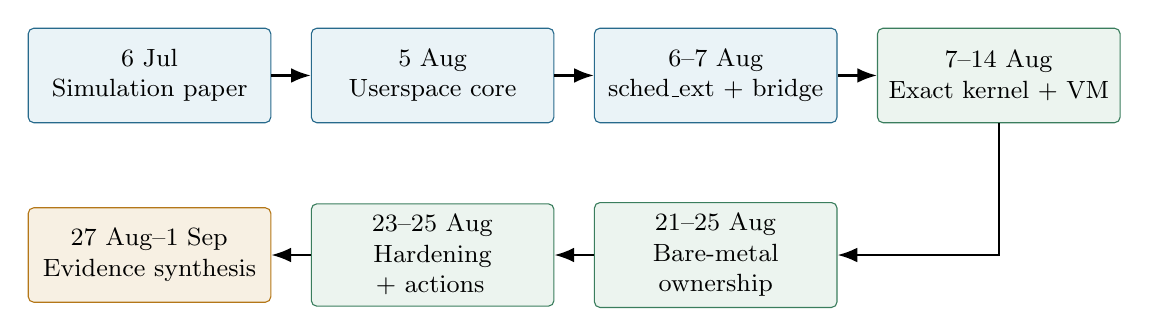
\begin{tikzpicture}[node distance=7mm and 5mm]
 \node[bluebox,text width=28mm] (paper) {6 Jul\\Simulation paper};
 \node[bluebox,right=of paper,text width=28mm] (user) {5 Aug\\Userspace core};
 \node[bluebox,right=of user,text width=28mm] (kernel) {6--7 Aug\\sched\_ext + bridge};
 \node[greenbox,right=of kernel,text width=28mm] (vm) {7--14 Aug\\Exact kernel + VM};
 \node[greenbox,below=10mm of kernel,text width=28mm] (bare) {21--25 Aug\\Bare-metal ownership};
 \node[greenbox,left=of bare,text width=28mm] (hard) {23--25 Aug\\Hardening + actions};
 \node[amberbox,left=of hard,text width=28mm] (synth) {27 Aug--1 Sep\\Evidence synthesis};
 \draw[arrow] (paper)--(user);
 \draw[arrow] (user)--(kernel);
 \draw[arrow] (kernel)--(vm);
 \draw[arrow] (vm.south) |- (bare.east);
 \draw[arrow] (bare)--(hard);
 \draw[arrow] (hard)--(synth);
\end{tikzpicture}
\caption{Development and validation progression. Color distinguishes design
and implementation, kernel validation, and evidence synthesis; it does not
indicate deployment readiness.}
\label{fig:timeline}
\end{figure}

\section{Implemented architecture}

\begin{figure}[H]
\centering
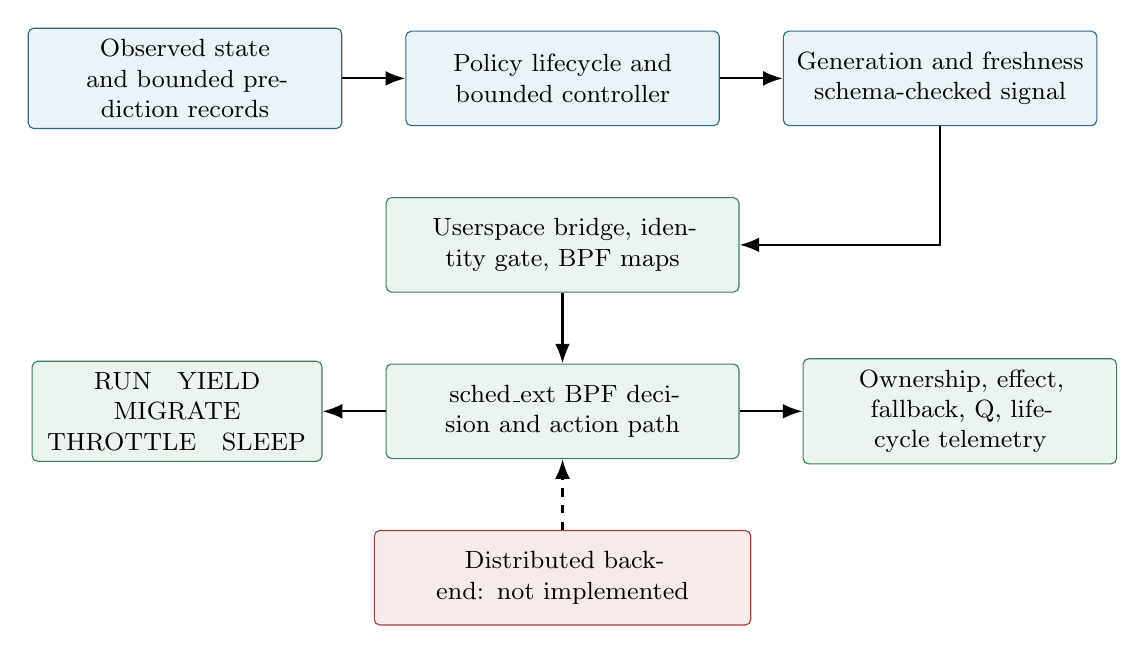
\begin{tikzpicture}[node distance=9mm and 8mm]
 \node[bluebox,text width=37mm] (state) {Observed state and bounded prediction records};
 \node[bluebox,right=of state,text width=37mm] (control) {Policy lifecycle and bounded controller};
 \node[bluebox,right=of control,text width=37mm] (signal) {Generation and freshness\\schema-checked signal};
 \node[greenbox,below=of control,text width=42mm] (bridge) {Userspace bridge, identity gate, BPF maps};
 \node[greenbox,below=of bridge,text width=42mm] (bpf) {sched\_ext BPF decision and action path};
 \node[greenbox,left=of bpf,text width=34mm] (actions) {RUN\quad YIELD\\MIGRATE\\THROTTLE\quad SLEEP};
 \node[greenbox,right=of bpf,text width=37mm] (tele) {Ownership, effect, fallback, Q, lifecycle telemetry};
 \node[redbox,below=of bpf,text width=45mm] (dist) {Distributed backend: not implemented};
 \draw[arrow] (state)--(control);
 \draw[arrow] (control)--(signal);
 \draw[arrow] (signal) |- (bridge);
 \draw[arrow] (bridge)--(bpf);
 \draw[arrow] (bpf)--(actions);
 \draw[arrow] (bpf)--(tele);
 \draw[arrow,dashed] (dist)--(bpf);
\end{tikzpicture}
\caption{Implemented single-host path and explicit non-implemented boundary.}
\label{fig:architecture}
\end{figure}

\begin{table}[H]
\centering
\caption{Research-to-product implementation matrix.}
\begin{tabularx}{\textwidth}{@{}p{35mm}p{45mm}Y@{}}
\toprule
\textbf{Component} & \textbf{Strongest evidence} & \textbf{Boundary} \\
\midrule
Scheduler, bridge, loader & Target verifier, attach, ownership, unload & One
target/API family; not general kernel portability. \\
Five action backends & Bounded real-machine action matrix & Not all workload,
fairness, topology, or timing conditions. \\
Signal bus & Userspace integrity and kernel generation/freshness gates & No HMAC
verifier in BPF. \\
Prediction & Confidence, expiry, generation, observed fallback contract &
Hardware prediction accuracy and benefit untested. \\
S1/S2/S3/S4/Q & Corrected contract and limited live windows & No broad
population statistical validation. \\
Controller & Bounded contract and limited transitions & Full causal actuator
and rollback matrix open. \\
RT boundary & Admission refusal and bounded FIFO/RR coexistence & No hard-RT
guarantee. \\
NUMA/distributed & One-node observation; no distributed backend & Cross-node
NUMA blocked; distributed tier absent. \\
\bottomrule
\end{tabularx}
\end{table}

\chapter{Validation Method and Evidence Quality}

\section{Evidence chain}

\begin{figure}[H]
\centering
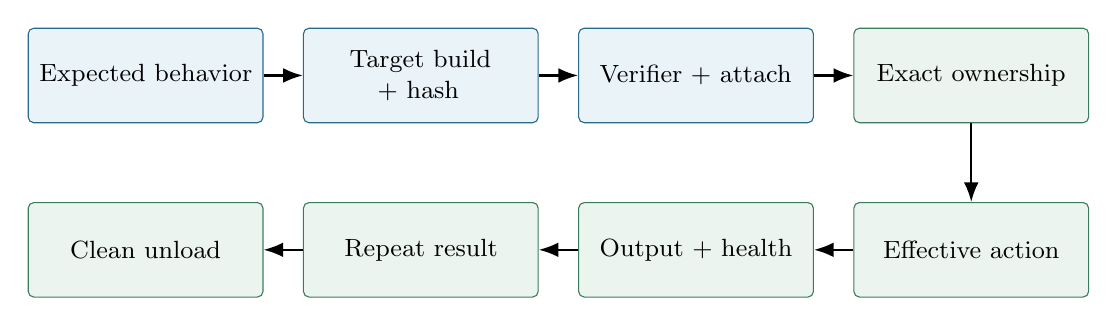
\begin{tikzpicture}[node distance=6mm and 5mm]
 \node[bluebox,text width=27mm] (spec) {Expected behavior};
 \node[bluebox,right=of spec,text width=27mm] (build) {Target build + hash};
 \node[bluebox,right=of build,text width=27mm] (attach) {Verifier + attach};
 \node[greenbox,right=of attach,text width=27mm] (own) {Exact ownership};
 \node[greenbox,below=10mm of own,text width=27mm] (effect) {Effective action};
 \node[greenbox,left=of effect,text width=27mm] (correct) {Output + health};
 \node[greenbox,left=of correct,text width=27mm] (repeat) {Repeat result};
 \node[greenbox,left=of repeat,text width=27mm] (close) {Clean unload};
 \draw[arrow] (spec)--(build);
 \draw[arrow] (build)--(attach);
 \draw[arrow] (attach)--(own);
 \draw[arrow] (own)--(effect);
 \draw[arrow] (effect)--(correct);
 \draw[arrow] (correct)--(repeat);
 \draw[arrow] (repeat)--(close);
\end{tikzpicture}
\caption{Evidence chain required for a bounded real-machine claim.}
\label{fig:evidence}
\end{figure}

\section{Checklist status}

\begin{figure}[H]
\centering
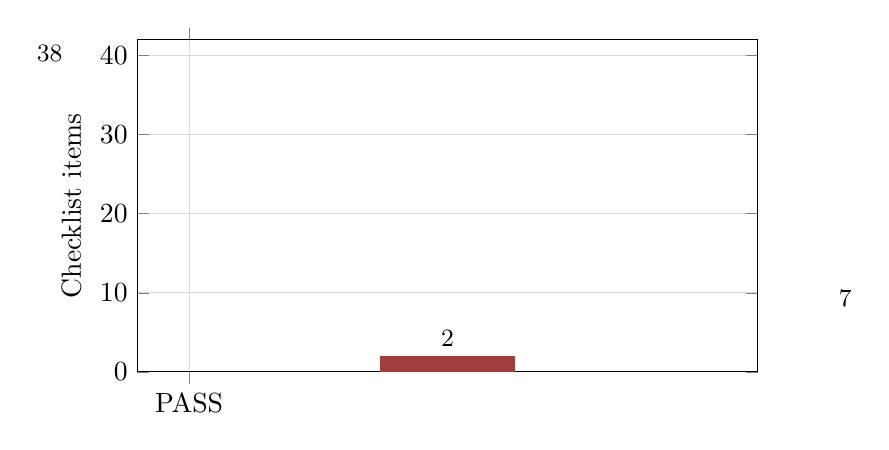
\begin{tikzpicture}
\begin{axis}[
 width=0.78\textwidth,height=58mm,ybar,bar width=17mm,
 symbolic x coords={PASS,FAIL,BLOCKED},xtick=data,
 ymin=0,ymax=42,ytick={0,10,20,30,40},ylabel={Checklist items},
 grid=major,major grid style={draw=gridgray},
 nodes near coords,every node near coord/.append style={font=\bfseries\small}
]
\addplot[draw=rgreen,fill=rgreen] coordinates {(PASS,38)};
\addplot[draw=rred,fill=rred] coordinates {(FAIL,2)};
\addplot[draw=ramber,fill=ramber] coordinates {(BLOCKED,7)};
\end{axis}
\end{tikzpicture}
\caption{Principal 47-item checklist. PASS applies only to the named bounded
test and does not upgrade blocked deployment claims.}
\label{fig:checklist}
\end{figure}

\section{Representative action evidence}

\begin{table}[H]
\centering
\caption{Bounded action observations from the 81/81 matrix.}
\begin{tabularx}{\textwidth}{@{}p{26mm}p{62mm}Y@{}}
\toprule
\textbf{Action} & \textbf{Observed evidence} & \textbf{Boundary} \\
\midrule
RUN & Dispatch 31; running 34; effective 34 & Controlled forward progress. \\
YIELD & 45 specialized dispatches; 44 effective; peer progress & Bounded
queue-tail behavior, not universal latency. \\
MIGRATE & 28 accepted; 28 dispatched; 27 effective; requested, dispatched, and
actual CPU all 1 & Same-node movement only. \\
Invalid MIGRATE & 44 bad-CPU fallbacks; zero MIGRATE acceptance or dispatch;
effective RUN fallback & Fail-closed for this invalid target. \\
SLEEP & Acceptance, defer, release, resumed progress & One-shot bounded
defer/release evidence. \\
THROTTLE & Immediate, after-RUN, rollover, republication, and two-CPU cases &
Broad fairness and bandwidth semantics remain open. \\
\bottomrule
\end{tabularx}
\end{table}

\chapter{Product Results}

\section{General fixed-work performance}

\begin{figure}[H]
\centering
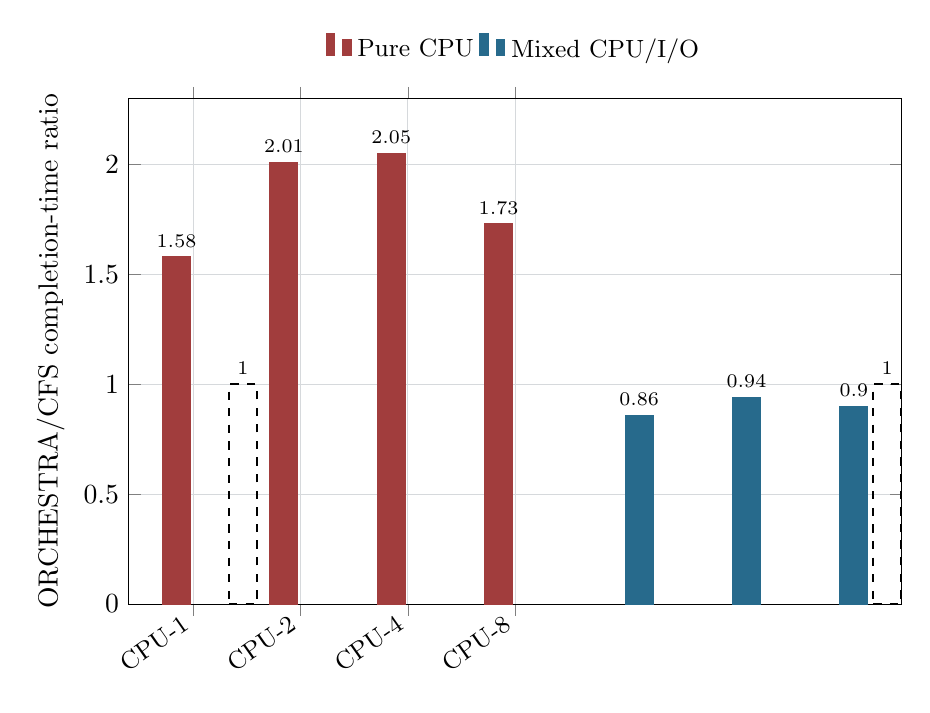
\begin{tikzpicture}
\begin{axis}[
 width=0.94\textwidth,height=80mm,ybar,bar width=10pt,
 symbolic x coords={CPU-1,CPU-2,CPU-4,CPU-8,MIX-1,MIX-2,MIX-4},
 xtick=data,x tick label style={rotate=35,anchor=east,font=\small},
 ylabel={ORCHESTRA/CFS completion-time ratio},
 ymin=0,ymax=2.3,ytick={0,0.5,1,1.5,2},
 grid=major,major grid style={draw=gridgray},
 nodes near coords,every node near coord/.append style={font=\scriptsize},
 legend style={font=\small,draw=none,at={(0.5,1.05)},anchor=south,legend columns=2}
]
\addplot[draw=rred,fill=rred] coordinates
 {(CPU-1,1.58) (CPU-2,2.01) (CPU-4,2.05) (CPU-8,1.73)};
\addplot[draw=rblue,fill=rblue] coordinates
 {(MIX-1,0.86) (MIX-2,0.94) (MIX-4,0.90)};
\addplot[black,dashed,thick,forget plot] coordinates {(CPU-1,1) (MIX-4,1)};
\legend{Pure CPU,Mixed CPU/I/O}
\end{axis}
\end{tikzpicture}
\caption{Fixed-work results, N=3 per scheduler per cell. Pure CPU is negative;
mixed CPU/I/O is directionally positive but exploratory.}
\label{fig:fixed}
\end{figure}

Pure CPU is the clearest performance weakness. A complete cause requires
matched \texttt{perf}, tracepoint, cache, and target-matched
\texttt{scx\_simple} evidence, which was unavailable.

\section{Strongest result: foreground protection}

The held-out protocol ran four foreground ImageMagick resizes with eight bzip2
background workers for 20 counterbalanced pairs. Output, ownership, effective
THROTTLE, and clean-unload gates passed.

\begin{figure}[H]
\centering
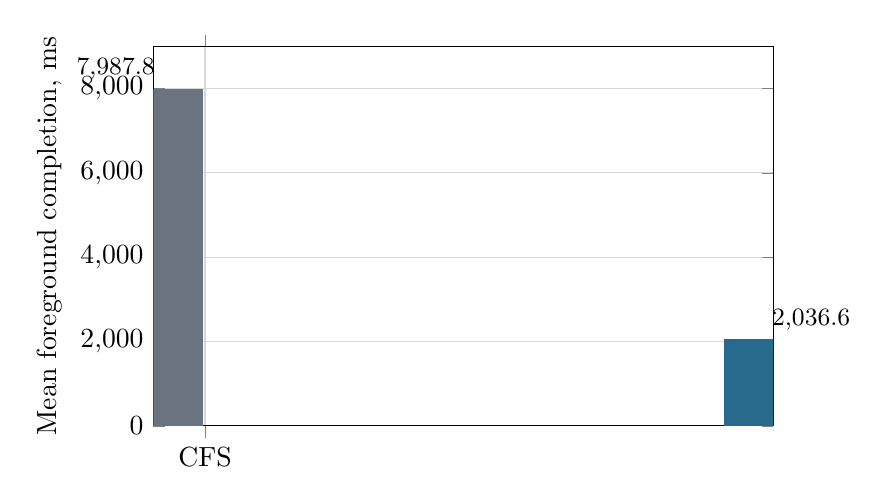
\begin{tikzpicture}
\begin{axis}[
 width=0.78\textwidth,height=64mm,ybar,bar width=22mm,
 symbolic x coords={CFS,ORCHESTRA},xtick=data,
 ymin=0,ymax=9000,ytick={0,2000,4000,6000,8000},
 ylabel={Mean foreground completion, ms},
 grid=major,major grid style={draw=gridgray},
 nodes near coords,every node near coord/.append style={font=\bfseries\small}
]
\addplot[draw=rgray,fill=rgray] coordinates {(CFS,7987.8)};
\addplot[draw=rblue,fill=rblue] coordinates {(ORCHESTRA,2036.6)};
\end{axis}
\end{tikzpicture}
\caption{Foreground means. ORCHESTRA won 20/20 pairs; mean paired reduction was
74.2405\%.}
\label{fig:foreground}
\end{figure}

\begin{figure}[H]
\centering
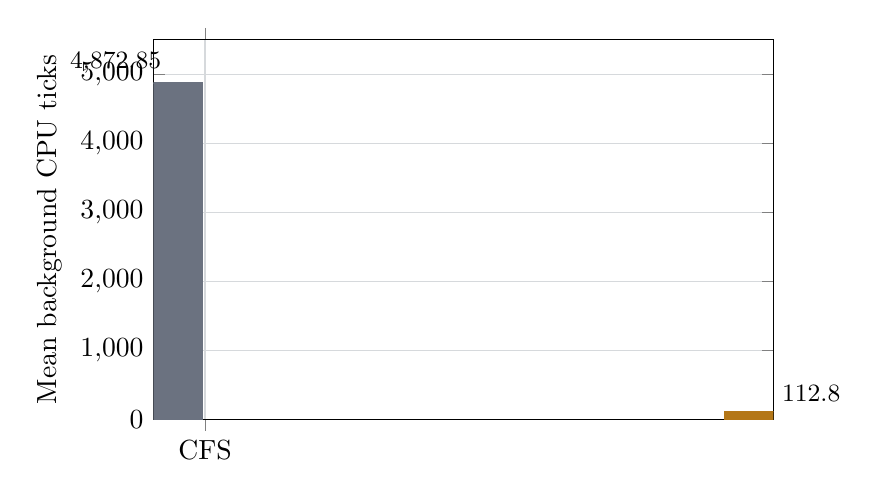
\begin{tikzpicture}
\begin{axis}[
 width=0.78\textwidth,height=64mm,ybar,bar width=22mm,
 symbolic x coords={CFS,ORCHESTRA},xtick=data,
 ymin=0,ymax=5500,ytick={0,1000,2000,3000,4000,5000},
 ylabel={Mean background CPU ticks},
 grid=major,major grid style={draw=gridgray},
 nodes near coords,every node near coord/.append style={font=\bfseries\small}
]
\addplot[draw=rgray,fill=rgray] coordinates {(CFS,4872.85)};
\addplot[draw=ramber,fill=ramber] coordinates {(ORCHESTRA,112.80)};
\end{axis}
\end{tikzpicture}
\caption{Service cost. Mean background CPU ticks fell 97.6851\%.}
\label{fig:cost}
\end{figure}

The graphs must be read together. ORCHESTRA protected foreground work by
restricting background service. Background completion, total makespan, and a
matched CFS cgroup or CPU-quota policy were not measured. This is service-policy
evidence, not proof of better total-system efficiency.

\section{Integrity, stress, and real-time boundary}

\begin{itemize}
 \item Userspace publication passed 12/12 runs, 12,000 publications, and 27,161
 verified reads. BPF contains no HMAC verifier.
 \item Ownership-gated CPU, I/O, and mixed phases ran 600 seconds each with no
 recorded errors or warnings and clean unload. Memory remained blocked.
 \item FIFO/RR coexistence preserved protected tasks outside the adaptive path.
 DEADLINE contention was blocked by host \texttt{EPERM}; hard RT is not proven.
 \item A log/archive result showed 5/5 wins and a 60.4678\% mean paired
 reduction, but 96--97\,$^\circ$C measurements make it thermally confounded.
\end{itemize}

\chapter{Engineering Discoveries}

\begin{enumerate}
 \item \textbf{Correctness is a chain, not a success message.} Build, verifier,
 attach, ownership, request, acceptance, dispatch, effect, fallback, and unload
 are distinct claims.
 \item \textbf{Exact kernel matching is a release constraint.} Kernel API, BTF,
 headers, toolchain, and loader identity must be recorded per target.
 \item \textbf{Observability is a product feature.} Requested-to-effective
 telemetry made stale generation, migration fallback, deferred release,
 controller state, and cleanup diagnosable.
 \item \textbf{Service policy differs from speed.} Background CPU service
 changed the interpretation of the foreground improvement.
 \item \textbf{Exact TID admission does not cover every application.} Some
 nominally single-threaded tools expose multiple active TIDs.
 \item \textbf{Transitions are high-risk.} A reproduced RUN-to-THROTTLE
 bottleneck showed the importance of generation and accounting synchronization.
 \item \textbf{Negative results improve credibility.} CPU slowdown, predictor
 failure, thermal confounding, one-node NUMA, and the absent distributed backend
 correctly narrowed the claim.
\end{enumerate}

\chapter{Strength and Weakness Assessment}

Ratings summarize evidence in this project, not personal intelligence or future
potential.

\begin{figure}[H]
\centering
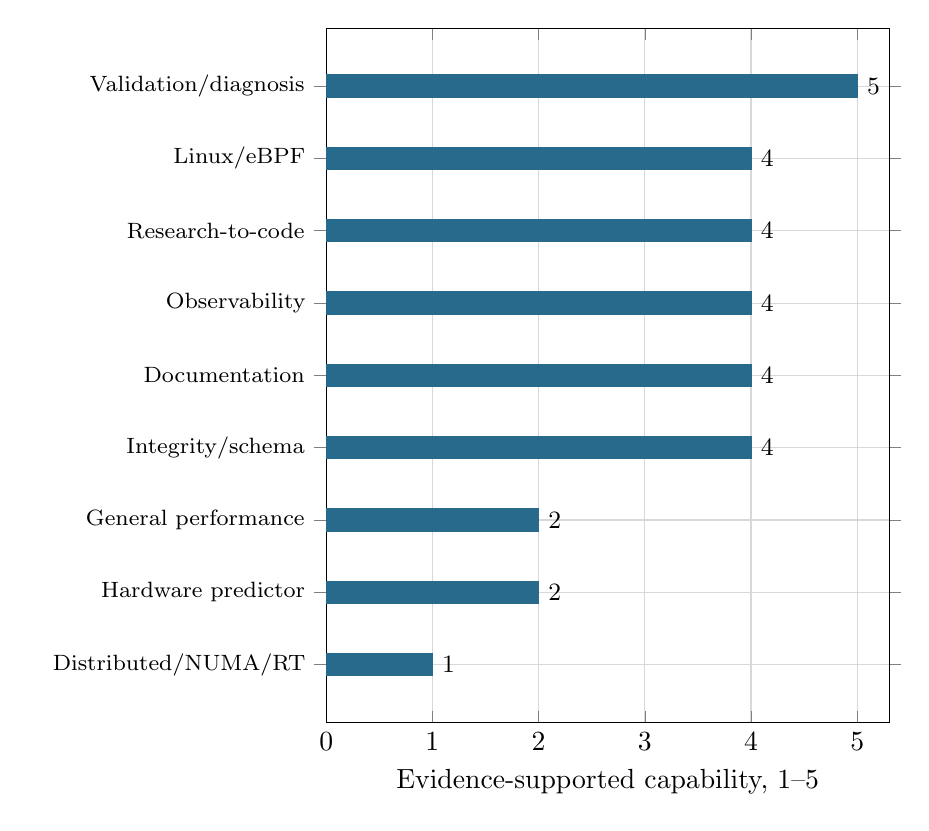
\begin{tikzpicture}
\begin{axis}[
 xbar,bar width=8pt,width=0.72\textwidth,height=104mm,
 xmin=0,xmax=5.3,xtick={0,1,2,3,4,5},
 xlabel={Evidence-supported capability, 1--5},
 symbolic y coords={Distributed/NUMA/RT,Hardware predictor,General performance,Integrity/schema,Documentation,Observability,Research-to-code,Linux/eBPF,Validation/diagnosis},
 ytick=data,y tick label style={font=\footnotesize,align=right,text width=34mm},
 grid=major,major grid style={draw=gridgray},
 nodes near coords,every node near coord/.append style={font=\small}
]
\addplot[draw=rblue,fill=rblue] coordinates {
 (1,Distributed/NUMA/RT)
 (2,Hardware predictor)
 (2,General performance)
 (4,Integrity/schema)
 (4,Documentation)
 (4,Observability)
 (4,Research-to-code)
 (4,Linux/eBPF)
 (5,Validation/diagnosis)
};
\end{axis}
\end{tikzpicture}
\caption{Capability assessment from direct repository evidence.}
\label{fig:strength}
\end{figure}

\section{Strongest areas}

\begin{enumerate}
 \item Evidence-led systems validation and diagnosis;
 \item Linux/eBPF and \schedext{} prototyping;
 \item research-to-code translation;
 \item observability, identity, fallback, and lifecycle design;
 \item reproducibility and formal technical communication; and
 \item controlled foreground service policy within one validated protocol.
\end{enumerate}

\section{Weak or incomplete areas}

\begin{itemize}
 \item Pure-CPU performance and context-switch cost;
 \item hardware predictor accuracy and measurable scheduling benefit;
 \item full controller-actuator causality and rollback;
 \item whole-application ownership for multithreaded software;
 \item kernel cryptographic authentication and key lifecycle; and
 \item hard RT, cross-node NUMA, hotplug, distributed scheduling, and production
 readiness.
\end{itemize}

\chapter{Professional and Work-Fit Assessment}

\section{Best-fit job families}

\begin{figure}[H]
\centering
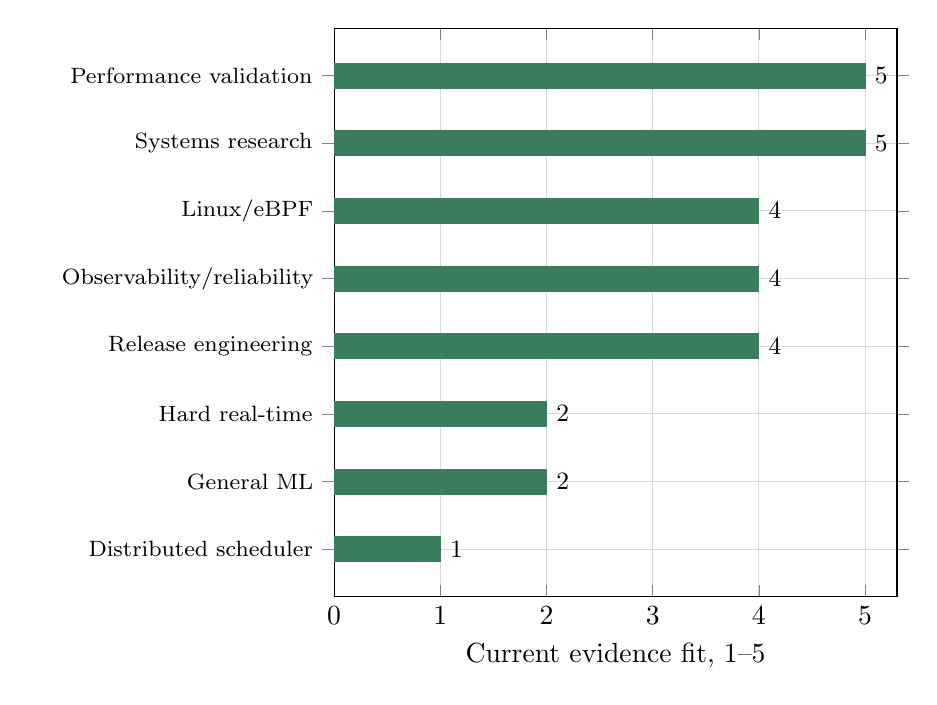
\begin{tikzpicture}
\begin{axis}[
 xbar,bar width=9pt,width=0.72\textwidth,height=88mm,
 xmin=0,xmax=5.3,xtick={0,1,2,3,4,5},
 xlabel={Current evidence fit, 1--5},
 symbolic y coords={Distributed scheduler,General ML,Hard real-time,Release engineering,Observability/reliability,Linux/eBPF,Systems research,Performance validation},
 ytick=data,y tick label style={font=\footnotesize,align=right,text width=35mm},
 grid=major,major grid style={draw=gridgray},
 nodes near coords,every node near coord/.append style={font=\small}
]
\addplot[draw=rgreen,fill=rgreen] coordinates {
 (1,Distributed scheduler)
 (2,General ML)
 (2,Hard real-time)
 (4,Release engineering)
 (4,Observability/reliability)
 (4,Linux/eBPF)
 (5,Systems research)
 (5,Performance validation)
};
\end{axis}
\end{tikzpicture}
\caption{Job-family fit based only on evidence demonstrated by ORCHESTRA-OS.}
\label{fig:jobs}
\end{figure}

\begin{longtable}{@{}p{46mm}C{20mm}p{83mm}@{}}
\caption{Professional fit and honest boundary.}\label{tab:jobs}\\
\toprule
\textbf{Job family} & \textbf{Fit} & \textbf{Evidence and boundary} \\
\midrule
\endfirsthead
\toprule
\textbf{Job family} & \textbf{Fit} & \textbf{Evidence and boundary} \\
\midrule
\endhead
Systems Research / Research Software Engineer & Excellent & Paper-to-prototype
translation, controlled experiments, and negative-result diagnosis. Describe it
as bounded, not production-ready. \\
Performance / Benchmarking Engineer & Excellent & Baselines, ownership,
counterbalancing, repetitions, confounder detection, and service-cost analysis.
Do not claim universal speed. \\
Linux Systems / eBPF Engineer & Strong & BPF maps, target matching, loader
lifecycle, \schedext{}, identity, and verifier-aware testing. Larger production
kernel coverage remains open. \\
Systems Validation Engineer & Excellent & Action, integrity, stress, RT
boundary, fault/recovery, and checklist evidence with preserved failures. \\
Observability / Reliability Engineer & Strong & Requested-to-effective
telemetry, lifecycle, fallbacks, health, and causal diagnosis. Production uptime
is not represented. \\
Edge Resource-Management Engineer & Strong & Opt-in service differentiation
and mixed CPU/I/O fit constrained worker pools. Field confirmation is required. \\
Native Build / Release Engineer & Good & Kernel manifests, ABI/schema gates,
hashes, packaging, and reproducibility. Cross-platform coverage remains open. \\
Hard RT / Distributed / NUMA-HPC / Crypto Assurance & Not yet supported &
Relevant implementation or validation is blocked, absent, or too narrow. \\
\bottomrule
\end{longtable}

\section{Best kinds of work}

The evidence suggests the team is best suited to projects where a research
architecture must become a bounded prototype; behavior crosses userspace and
kernel boundaries; instrumentation is as important as implementation; failures
must be reproduced and explained; and identity, safety, fallback, lifecycle,
and reproducibility matter.

Suitable work includes eBPF policy engines, kernel observability tools, resource
governors, edge workload controllers, systems test platforms, fault/recovery
harnesses, native-software release pipelines, and research prototypes.

\section{Defensible portfolio statement}

\begin{quote}
Built and validated a research-grade, opt-in Linux \schedext{} control and
observability prototype that translated predictive scheduling research into
five bounded kernel actions with exact ownership, fallback, and lifecycle
evidence.
\end{quote}

\textbf{Claims to avoid:} ORCHESTRA is faster than Linux; deployment ready;
kernel signal authentication is proven; hard real-time is proven; distributed
scheduling is implemented; or prediction improves hardware scheduling.

\chapter{Recommendations and Roadmap}

\section{Highest-value next experiment}

The next decisive test is a matched service-policy comparison, not another
broad demonstration.

\begin{figure}[H]
\centering
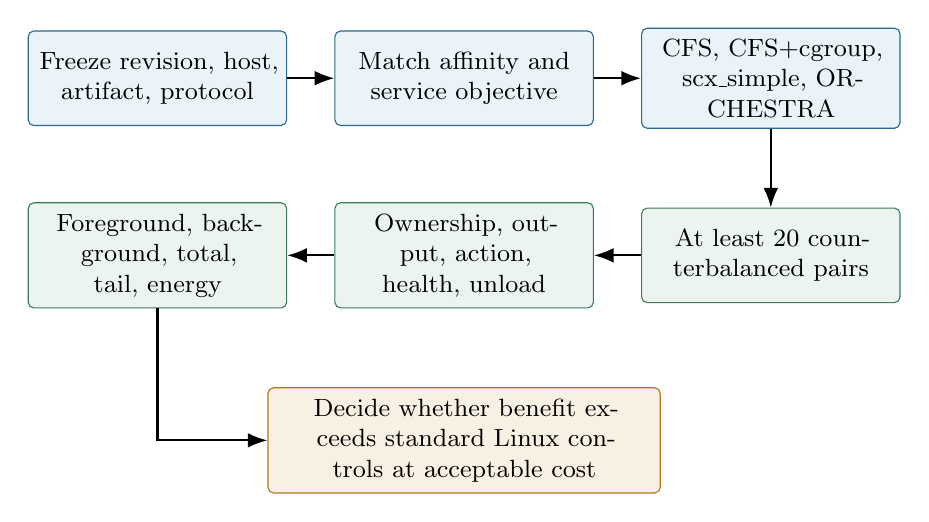
\begin{tikzpicture}[node distance=7mm and 6mm]
 \node[bluebox,text width=30mm] (freeze) {Freeze revision, host, artifact, protocol};
 \node[bluebox,right=of freeze,text width=30mm] (baseline) {Match affinity and service objective};
 \node[bluebox,right=of baseline,text width=30mm] (modes) {CFS, CFS+cgroup, scx\_simple, ORCHESTRA};
 \node[greenbox,below=10mm of modes,text width=30mm] (trials) {At least 20 counterbalanced pairs};
 \node[greenbox,left=of trials,text width=30mm] (gates) {Ownership, output, action, health, unload};
 \node[greenbox,left=of gates,text width=30mm] (metrics) {Foreground, background, total, tail, energy};
 \node[amberbox,below=10mm of gates,text width=47mm] (decision) {Decide whether benefit exceeds standard Linux controls at acceptable cost};
 \draw[arrow] (freeze)--(baseline);
 \draw[arrow] (baseline)--(modes);
 \draw[arrow] (modes)--(trials);
 \draw[arrow] (trials)--(gates);
 \draw[arrow] (gates)--(metrics);
 \draw[arrow] (metrics) |- (decision);
\end{tikzpicture}
\caption{Recommended evidence path for the next product decision.}
\label{fig:roadmap}
\end{figure}

\begin{table}[H]
\centering
\caption{Priority gap-closure plan.}
\begin{tabularx}{\textwidth}{@{}C{12mm}p{38mm}Yp{34mm}@{}}
\toprule
\textbf{P} & \textbf{Gap} & \textbf{Required evidence} & \textbf{Claim unlocked} \\
\midrule
1 & Matched policy baseline & CFS+cgroup and ORCHESTRA with identical service
objectives and at least 20 pairs & Value beyond standard Linux controls. \\
2 & CPU overhead & \texttt{perf}, tracepoints, callbacks, migrations, cache
misses, and matched \texttt{scx\_simple} & Causal overhead diagnosis. \\
3 & Whole-application ownership & Thread-group or cgroup admission and
per-thread telemetry & Defensible application control. \\
4 & Predictor/controller & Dynamic regimes, error, confidence, actuator
response, saturation, rollback & Hardware predictive/control evidence. \\
5 & Kernel trust boundary & Threat model, key lifecycle, provenance, fuzzing,
independent review & Narrow secure-system claim. \\
6 & Platform maturity & Multi-node NUMA, hotplug, x86/arm matrix, long soak,
upgrade and rollback & Broader release readiness. \\
\bottomrule
\end{tabularx}
\end{table}

\chapter{Final Conclusion}

ORCHESTRA-OS has achieved more than a paper reproduction and less than a
production scheduler. It has a coherent research-to-code mapping, a
target-specific working \schedext{} prototype, exact ownership and action
evidence, strong observability, bounded stress and recovery evidence, and a
reproducible foreground service-control result.

It has not demonstrated a general CFS/EEVDF performance advantage, hardware
predictor benefit, kernel-side cryptographic verification, broad fairness or
tail latency, hard-RT safety, cross-node NUMA, distributed scheduling, or
deployment readiness.

\begin{center}
\fbox{\begin{minipage}{0.9\textwidth}
\large
ORCHESTRA-OS is a research-grade, opt-in Linux scheduler control and
observability platform with bounded real-machine validation of ownership, five
actions, fallback, lifecycle, and foreground service protection. General
performance and production-readiness claims remain open.
\end{minipage}}
\end{center}

The strongest professional story is that the team took an ambitious
operating-systems research architecture, identified where its assumptions
failed, translated its strongest ideas into a real Linux/eBPF prototype, proved
what the kernel did, preserved negative results, and defined the evidence
required for the next product claim.

\appendix
\chapter{Evidence Reference Register}

\small
\begin{thebibliography}{99}
\bibitem{paper}
G. Ganesan and P. Vaithiyanathan,
\emph{ORCHESTRA-OS: Simulation-Driven Architectural Discovery and Design
Principles for Predictive, Hierarchical, Signal-Coordinated Process Scheduling},
6 July 2026. Repository PDF SHA-256:
\texttt{9af8f45412e2f7d8be89f108965372caa2c420f917c7b612c3b4a86ab626561d}.

\bibitem{wp}
ORCHESTRA-OS, \emph{Work Package Description},
\texttt{WORK\_PACKAGE\_DESCRIPTION.md}.

\bibitem{mapping}
ORCHESTRA-OS, \emph{Research-to-Code Mapping},
\texttt{docs/research/RESEARCH\_TO\_CODE.md}.

\bibitem{status}
ORCHESTRA-OS, \emph{Final Product Status},
\texttt{FINAL\_PRODUCT\_STATUS.md}.

\bibitem{validation}
S.W. ZAW, \emph{ORCHESTRA-OS versus Linux CFS: Validation Report Package},
1 September 2026, including provenance, audit, evidence calculations,
implementation matrix, checklist, action matrix, fixed-work data, paired
foreground statistics, long-run results, and checksums.

\bibitem{fit}
S.W. ZAW, \emph{ORCHESTRA-OS Real-World Field-Fit Report}, 27 August 2026.

\bibitem{strength}
S.W. ZAW, \emph{ORCHESTRA-OS Strongest Part and Real-World Comparison Guide},
27 August 2026.
\end{thebibliography}

\chapter{Reproducibility Note}

No new scheduler run was performed to create this report. Numerical claims were
taken from the frozen validation package whose audit records successful
checksum verification and recalculation. Because the current worktree contains
staged and untracked changes, a future campaign must freeze a new revision,
capture repository and machine state, rebuild the exact target artifact, and
repeat the relevant gates.

\end{document}
